%!TEX root = ../thesis.tex

\section{Deep learning}
Deep learningは, 画像や音声などのデータに特に適しており, 近年では
自然言語処理や医療画像解析などさまざまな分野で活用されている.
人間の脳のような深い層の構造を持つ人工ニューラルネットワークに基づく機械学習手法である. 
人工ニューラルネットワークは, 入力データから出力データを予測するために, 多数のニューロンを
用いて情報を処理する. この人工ニューラルネットワークを多層構造にすることで, より深い情報
処理を行うことができる. これにより, 高度な識別や分類タスクなどを行うことを可能にしている. 
一般的な構造を\ref{Fig:Neural network} に示す.

% \subsection{RoboCup}

\begin{figure}[hbtp]
  \centering
 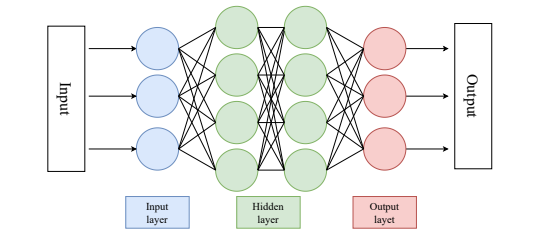
\includegraphics[keepaspectratio, scale=0.4]
      {images/deeplearning_model.png}
 \caption{Neural network}
 \label{Fig:Neural network}
\end{figure}

% \subsubsection{etc...}
\newpage
